%TD -- Kapitel 4.3 -- alle Labels darauf aufbauend

\newpage
\section{Lautsprecher für Hochton-Bereich}\label{sec:4.3}
Je ein Hochton-Lautsprecher wird in eine Satelliten-Box verbaut.
Während für die Tiefton-Lautsprecher das Volumen noch sehr wichtig ist, weil es den Frequenzgang des Lautsprechers beeinflussen kann, spielt das Volumen für die Hochton-Lautsprecher keine große Rolle mehr.
Dies ist bedingt dadurch, dass der Schall des Hochton-Lautsprecher sich hauptsächlich in Abstrahlrichtung der Membran ausbreitet.
%Das kommt daher, dass der Schall nur aus Richtung der Hochton-Lautsprecher-Membran abgestrahlt wird.
Die Box wird also durch hohe Töne nicht in Schwingung versetzt.
\\ \\
Folgende Hochton-Lautsprecher wurden gemessen:
\begin{itemize}
	\item TW203
	\item AE-1004
	\item Sharp 50T
	\item DT4810ASZR
	\item U2275
	\item Visaton DTW72 (zugekauft)
\end{itemize}
Um vergleichbare Messungen zu erhalten, wurden alle Hochton-Lautsprecher mit einer Entfernung von 1 m zum Mikrofon gemessen.
Außerdem wurden alle Lautsprecher in einer Höhe von 1 m platziert, um Reflexionen mit dem Boden des Messraums zu verhindern.
Vor allem aus dem Grund, da es sich bei dem Boden um ein Metallgitter handelt.
In den Auslassungen des Gitters könnte es zu möglichen Resonanzen oder Reflexionen kommen, die das Messergebnis verfälschen.
\newpage

\begin{figure} [H]
	\centering
	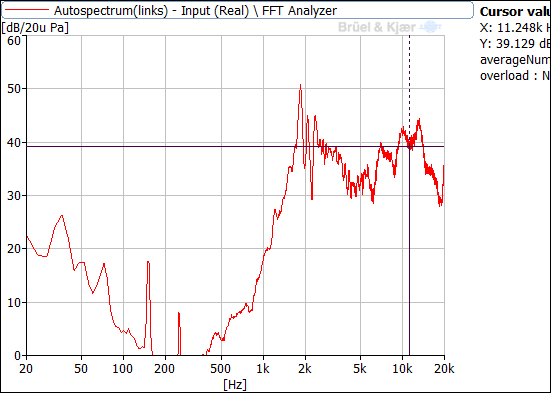
\includegraphics[width=0.8\textwidth]{img/LSMessung/HT/TW203_1m_erhoeht.png}
	\caption{Frequenzgang \enquote{TW203}}
	\label{fig:4.3.1}
\end{figure}

\begin{figure} [H]
	\centering
	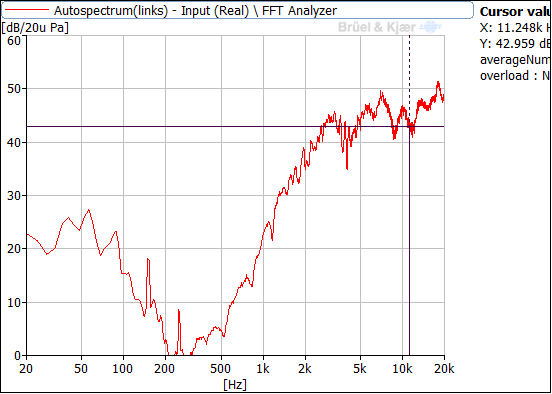
\includegraphics[width=0.8\textwidth]{img/LSMessung/HT/AE1004_1m_erhoeht.png}
	\caption{Frequenzgang \enquote{AE-1004}}
	\label{fig:4.3.2}
\end{figure}

\begin{figure} [H]
	\centering
	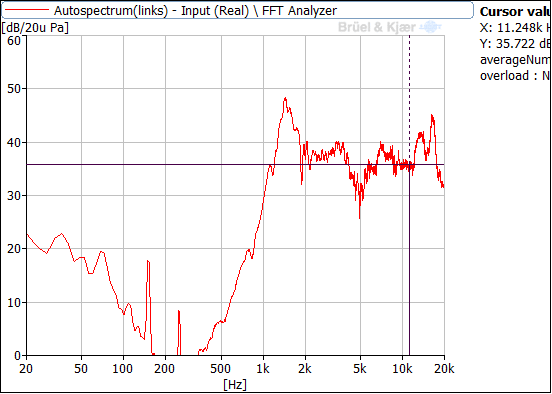
\includegraphics[width=0.8\textwidth]{img/LSMessung/HT/Sharp_1m_erhoeht.png}
	\caption{Frequenzgang \enquote{Sharp 50T}}
	\label{fig:4.3.3}
\end{figure}

\begin{figure} [H]
	\centering
	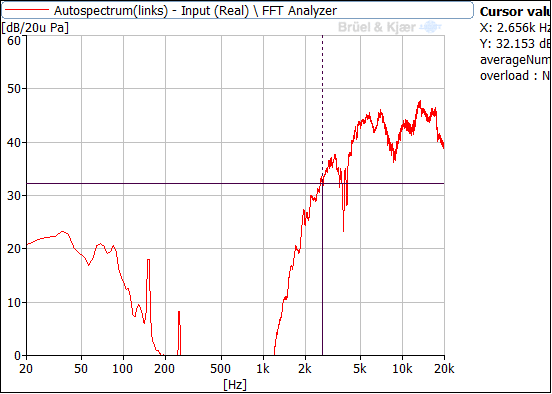
\includegraphics[width=0.8\textwidth]{img/LSMessung/HT/DT4810ASZR_1m_erhoeht.png}
	\caption{Frequenzgang \enquote{DT4810AZSR}}
	\label{fig:4.3.4}
\end{figure}

\begin{figure} [H]
	\centering
	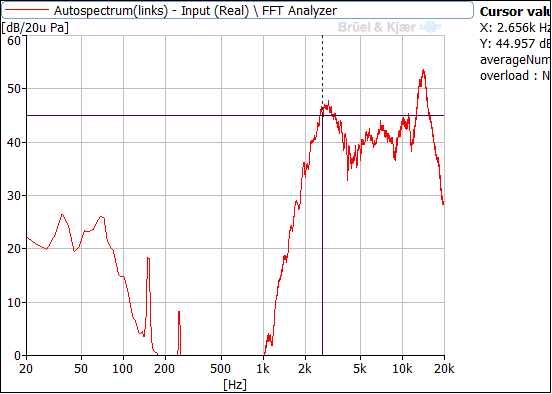
\includegraphics[width=0.8\textwidth]{img/LSMessung/HT/U2275_1m_erhoeht.png}
	\caption{Frequenzgang \enquote{U2275}}
	\label{fig:4.3.5}
\end{figure}

\begin{figure} [H]
	\centering
	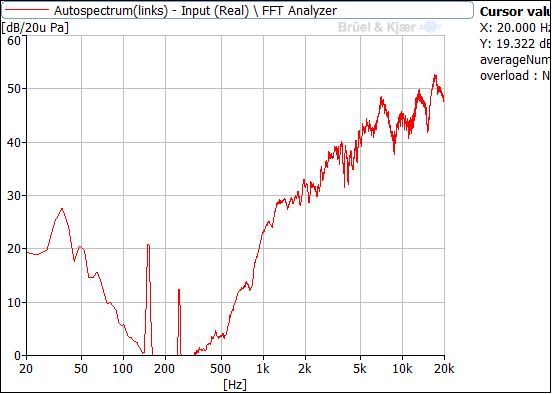
\includegraphics[width=0.8\textwidth]{img/LSMessung/HT/VisatonDTW72.png}
	\caption{Frequenzgang \enquote{Visaton DTW72}}
	\label{fig:4.3.6}
\end{figure}
\newpage
Im Bereich unter 500 Hz sind bei den Messungen relativ hohe Pegel aufgetreten.
In diesem Frequenzbereich kann ein Hochton-Lautsprecher aber nicht solche Schalldruckpegel erzeugen, dafür ist die Membranfläche zu klein.
Daraus ist zu schließen, dass diese Pegel durch verschiedene Störeinflüsse auf die Messung erzeugt wurden.
Diese Einflüsse könnten sein: Beeinflussung der Messung durch das 50 Hz Stromnetz, äußere Einflüsse auf den nahezu schalldichten Raum (Trittschall), usw.
\\ \\
Da viele dieser gemessenen Frequenzgänge eine hohe Welligkeit oder erst bei relativ hohen Frequenzen einen angemessenen Schalldruckpegel aufweisen, wurde von uns der Hochton-Lautsprecher \enquote{Visaton DTW72} (Frequenzgang: Abb. \ref{fig:4.3.6}) zugekauft und für das Projekt ausgewählt.
\\ \\
Dieser Lautsprecher weist einen angemessenen Schalldruckpegel bei relativ geringer Welligkeit auf und ist daher optimal.
Außerdem könnte er bereits ab ca. 1 kHz verwendet werden.

\begin{figure} [H]
	\centering
	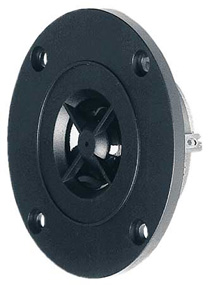
\includegraphics[width=0.4\textwidth]{img/LSMessung/HT/dtw72.jpg}
	\caption[Lautsprecher \enquote{Visaton DTW72}]{Lautsprecher \enquote{Visaton DTW72}\footnotemark}
	\label{fig:4.3.7}
\end{figure}
\footnotetext{http://www.visaton.de/de/chassis\_zubehoer/ht\_kalotten/dtw72\_8.html,\\Zugriff: 13.03.2017}
%http://www.visaton.de/de/chassis_zubehoer/ht_kalotten/dtw72_8.html
